\documentclass[aspectratio=169]{beamer}

\usepackage[english]{babel}
\usepackage{graphicx}
\usepackage{media9}
\usepackage[absolute, overlay]{textpos}
\usepackage{multicol}
\usepackage{tikz}

\usetheme{Madrid}
\usecolortheme{crane}
\setbeamertemplate{page number in head/foot}{}
\setbeamertemplate{navigation symbols}{}

\title{Automatic Generation of Safety-Critical Test Scenarios\\for Collision Avoidance of Road Vehicles}
\author{Matthias Althoff and Sebastian Lutz}
\institute{University of Passau}
\date{\today}
\titlegraphic{
\includegraphics[height=.10\textheight]{media/logoUniPassau.jpg}}

\newcommand{\includeFSVideo}[1]{%
    \begin{textblock*}{5pt} (0pt, 0pt)
        \includemedia[
            height=\paperheight,
            width=\paperwidth,
            addresource=#1,
            activate=pageopen,
            flashvars={source=#1&autoPlay=true&loop=true}
        ]{}{VPlayer9.swf}
    \end{textblock*}
}

\newcommand{\videoframe}[1]{%
    \begin{frame}[plain]
        \includeFSVideo{#1}
    \end{frame}
}

\begin{document}

\begin{frame}[plain]
    \noindent\makebox[\textwidth]{%
        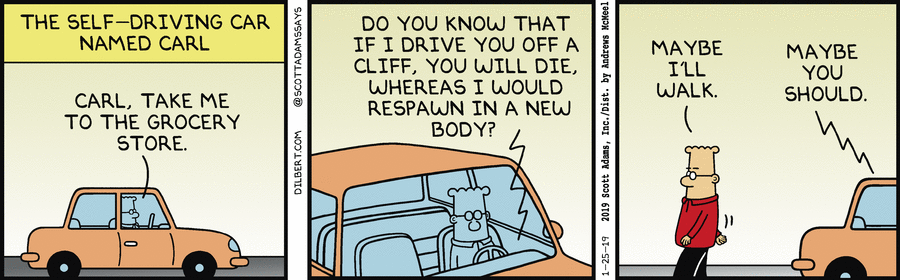
\includegraphics[width=.97\paperwidth]{media/2019-01-25_dilbert_autonomousCars.png}
    }
\end{frame}

\maketitle

\begin{frame}{Differentiation to other approaches}
    \begin{multicols}{2}
        Other approaches:
        \begin{tikzpicture}
            \node[anchor=south west, inner sep=0] at (0,0) {
\includegraphics[height=.9\textheight]{media/binoculars.jpg}};
            \onslide<2->{%
                \draw[red, line width=0.8mm, line cap=round] (0,1.5) -- (6.5,7) {};
                \draw[red, line width=0.8mm, line cap=round] (0,7) -- (6.5,1.5) {};
            }
        \end{tikzpicture}
        \vfill\null%
        \columnbreak%

        \pause%
        This approach:
        
\includegraphics[height=.9\textheight]{media/maurer.jpg}
    \end{multicols}
\end{frame}

\begin{frame}{Measurement of criticality}
\end{frame}

\videoframe{media/beamNG_toSlow.mp4}
\videoframe{media/beamNG_adequate.mp4}
\videoframe{media/beamNG_toFast.mp4}
%\videoframe{media/beamNG_adequate_freeView.mp4}
\videoframe{media/drivableArea_development.mp4}

\begin{frame}{Analyze development of drivable area}
    \begin{tikzpicture}
        \node[anchor=south west,inner sep=0] at (0,0) {\includegraphics[height=.95\textheight, trim=700 0 130 90, clip]{media/drivableArea_development.png}};
        % \draw[red,thick,rounded corners]5 (3.7,5.7) rectangle (4.8,6.2);
        \onslide<2->{%
            \draw[red] (3.84,5.85) circle (1.6pt) node[anchor=west];
            \draw[red, dashed] (3.84,5.7) -- (3.84,1);
            \draw[red] (4.025,5.85) circle (1.6pt) node[anchor=west];
            \draw[red, dashed] (4.025,5.7) -- (4.025,1);
            \draw[red] (4.56,5.81) circle (1.6pt) node[anchor=west];
            \draw[red, dashed] (4.56,5.7) -- (4.56,1);
        }
    \end{tikzpicture}
\end{frame}

\end{document}
